\documentclass[journal, a4paper]{IEEEtran}

% some very useful LaTeX packages include:

\usepackage{cite}      % Written by Donald Arseneau
                        % V1.6 and later of IEEEtran pre-defines the format
                        % of the cite.sty package \cite{} output to follow
                        % that of IEEE. Loading the cite package will
                        % result in citation numbers being automatically
                        % sorted and properly "ranged". i.e.,
                        % [1], [9], [2], [7], [5], [6]
                        % (without using cite.sty)
                        % will become:
                        % [1], [2], [5]--[7], [9] (using cite.sty)
                        % cite.sty's \cite will automatically add leading
                        % space, if needed. Use cite.sty's noadjust option
                        % (cite.sty V3.8 and later) if you want to turn this
                        % off. cite.sty is already installed on most LaTeX
                        % systems. The latest version can be obtained at:
                        % http://www.ctan.org/tex-archive/macros/latex/contrib/supported/cite/

\usepackage{graphicx}   % Written by David Carlisle and Sebastian Rahtz
                        % Required if you want graphics, photos, etc.
                        % graphicx.sty is already installed on most LaTeX
                        % systems. The latest version and documentation can
                        % be obtained at:
                        % http://www.ctan.org/tex-archive/macros/latex/required/graphics/
                        % Another good source of documentation is "Using
                        % Imported Graphics in LaTeX2e" by Keith Reckdahl
                        % which can be found as esplatex.ps and epslatex.pdf
                        % at: http://www.ctan.org/tex-archive/info/
\graphicspath{ {images/} }
\usepackage{tikz}
%\usepackage{psfrag}    % Written by Craig Barratt, Michael C. Grant,
                        % and David Carlisle
                        % This package allows you to substitute LaTeX
                        % commands for text in imported EPS graphic files.
                        % In this way, LaTeX symbols can be placed into
                        % graphics that have been generated by other
                        % applications. You must use latex->dvips->ps2pdf
                        % workflow (not direct pdf output from pdflatex) if
                        % you wish to use this capability because it works
                        % via some PostScript tricks. Alternatively, the
                        % graphics could be processed as separate files via
                        % psfrag and dvips, then converted to PDF for
                        % inclusion in the main file which uses pdflatex.
                        % Docs are in "The PSfrag System" by Michael C. Grant
                        % and David Carlisle. There is also some information
                        % about using psfrag in "Using Imported Graphics in
                        % LaTeX2e" by Keith Reckdahl which documents the
                        % graphicx package (see above). The psfrag package
                        % and documentation can be obtained at:
                        % http://www.ctan.org/tex-archive/macros/latex/contrib/supported/psfrag/

%\usepackage{subfigure} % Written by Steven Douglas Cochran
                        % This package makes it easy to put subfigures
                        % in your figures. i.e., "figure 1a and 1b"
                        % Docs are in "Using Imported Graphics in LaTeX2e"
                        % by Keith Reckdahl which also documents the graphicx
                        % package (see above). subfigure.sty is already
                        % installed on most LaTeX systems. The latest version
                        % and documentation can be obtained at:
                        % http://www.ctan.org/tex-archive/macros/latex/contrib/supported/subfigure/

\usepackage{url}        % Written by Donald Arseneau
                        % Provides better support for handling and breaking
                        % URLs. url.sty is already installed on most LaTeX
                        % systems. The latest version can be obtained at:
                        % http://www.ctan.org/tex-archive/macros/latex/contrib/other/misc/
                        % Read the url.sty source comments for usage information.
%\usepackage{stfloats}  % Written by Sigitas Tolusis
                        % Gives LaTeX2e the ability to do double column
                        % floats at the bottom of the page as well as the top.
                        % (e.g., "\begin{figure*}[!b]" is not normally
                        % possible in LaTeX2e). This is an invasive package
                        % which rewrites many portions of the LaTeX2e output
                        % routines. It may not work with other packages that
                        % modify the LaTeX2e output routine and/or with other
                        % versions of LaTeX. The latest version and
                        % documentation can be obtained at:
                        % http://www.ctan.org/tex-archive/macros/latex/contrib/supported/sttools/
                        % Documentation is contained in the stfloats.sty
                        % comments as well as in the presfull.pdf file.
                        % Do not use the stfloats baselinefloat ability as
                        % IEEE does not allow \baselineskip to stretch.
                        % Authors submitting work to the IEEE should note
                        % that IEEE rarely uses double column equations and
                        % that authors should try to avoid such use.
                        % Do not be tempted to use the cuted.sty or
                        % midfloat.sty package (by the same author) as IEEE
                        % does not format its papers in such ways.

\usepackage{amsmath}    % From the American Mathematical Society
                        % A popular package that provides many helpful commands
                        % for dealing with mathematics. Note that the AMSmath
                        % package sets \interdisplaylinepenalty to 10000 thus
                        % preventing page breaks from occurring within multiline
                        % equations. Use:
%\interdisplaylinepenalty=2500
                        % after loading amsmath to restore such page breaks
                        % as IEEEtran.cls normally does. amsmath.sty is already
                        % installed on most LaTeX systems. The latest version
                        % and documentation can be obtained at:
                        % http://www.ctan.org/tex-archive/macros/latex/required/amslatex/math/

\usepackage{gensymb}

% Other popular packages for formatting tables and equations include:

%\usepackage{array}
% Frank Mittelbach's and David Carlisle's array.sty which improves the
% LaTeX2e array and tabular environments to provide better appearances and
% additional user controls. array.sty is already installed on most systems.
% The latest version and documentation can be obtained at:
% http://www.ctan.org/tex-archive/macros/latex/required/tools/

% V1.6 of IEEEtran contains the IEEEeqnarray family of commands that can
% be used to generate multiline equations as well as matrices, tables, etc.

% Also of notable interest:
% Scott Pakin's eqparbox package for creating (automatically sized) equal
% width boxes. Available:
% http://www.ctan.org/tex-archive/macros/latex/contrib/supported/eqparbox/

% *** Do not adjust lengths that control margins, column widths, etc. ***
% *** Do not use packages that alter fonts (such as pslatex).         ***
% There should be no need to do such things with IEEEtran.cls V1.6 and later.
\usepackage{float}
\usepackage[justification=centering]{caption}

% Your document starts here!
\begin{document}

% Define document title and author
    \title{Beaver Works Summer Program Technical Report}
    \author{Michelle Tan}
    \maketitle

% Write abstract here
\begin{abstract}
    This material is part of a summer boot camp at MIT Beaver Works where teams of high schoolers compete in the Mini Grand Prix Challenge, an autonomous car race around a track. This program, which is based off the 6.141 Robotics Science and Systems class at MIT and the Robotics IAP, meets on weekdays for eight hours for four weeks. Each day typically consists of three lab periods, a technical lecture, a seminar with guest speakers, and an occasional communications class. 
\end{abstract}
% Each section begins with a \section{title} command
\section{Introduction}
    % \PARstart{}{} creates a tall first letter for this first paragraph
    \IEEEPARstart{T}{he} purpose of this program is to begin to understand the algorithms and methods used today in autonomous navigation and experiment with them on a 1/10-scale racecar. Teams could explore the abilities and limitations in building robust yet fast robotics systems. Some of the tasks given include following a wall, detecting a colored blob, following a colored blob, reactive obstacle detection, using a color to decide whether to take a turn, and optionally implementing localization and mapping. Much of the class dealt with how to deal with problems inherent to autonomous navigation, like sensor imperfections, object detection from camera images, and speed constraints. The cars used were referred to as RACECAR, which stands for Rapid Autonomous Complex-Environment Competing Ackermann-steering Robot. The cars were pre-built with it’s components prior to the start of the program, which includes the NVIDIA quad-core CPU, the 192-core GPU, an Ackermann-steering system, and a large variety of sensors including a Lidar, camera, and odometer. The teams used ROS, a “meta” operating system for robots that focuses on modularity, interfaces, and code reuse. \cite{plecture2} 
% Main Part
\section{Week 1}
\subsection{Technical Goal}
In the first week, the learning objective was to get experience in working with the sensors and actuation of the robot and learn about control systems. The end-of-week challenge consisted of being able to follow a left and right wall at a desired distanced away starting at various points away from the wall. 
\subsection{Approach}
The teams were required to use a Lidar to sense the wall but they were free to implement a state controller of their choice. [Go into details about state controllers]
\subsubsection{Bang Bang Controller}The simplest of the methods was using a Bang Bang controller, which would sense if the robot was too close or too far and if it was too close, it would turn away and if too far, turn towards. 
\subsubsection{PID Controller}A slightly more sophisticated version was to implement a PID(Proportional Integral Derivative) controller which does calculations on the error value to create a smooth oscillation to correct for the robot’s distance. In addition, for calculating the error distance, there was an additional consideration of which laser scan data to use. The angle of the robot could easily throw off the reading if only one measurement were taken, since the distance measured perpendicular from the robot won't necessarily be the true distance as shown below. \\ 
\begin{figure}[H]
\centering
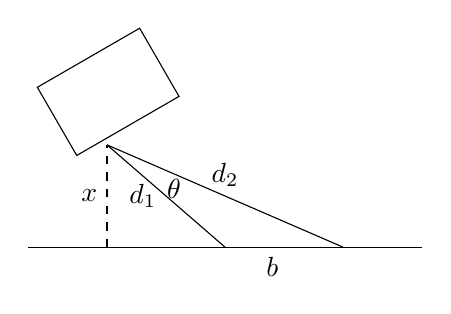
\begin{tikzpicture}
\draw[rotate around={30:(-1, 0.5)}] (0,3) rectangle(1.5,4);
\draw (-2,2)--(3,2) node at (1.1,2) [below] {$b$};
\draw [dashed] (-1,2)--(-1,3.3) node[midway, left]{$x$};
\draw (-1,3.3)--(0.5,2) node[midway, left]{$d_1$};
\draw (-1,3.3)--(2,2) node[midway, above]{$d_2$};
\draw node at (-0.15,2.5) [above] {$\theta$};
\end{tikzpicture}
\caption{Diagram of robot}
\end{figure}
A two point controller could account for this with basic trigonometry. Given two arbitrary angles to take the laser measurements $d_1$ and $d_2$, if the angle $\theta$ is known the following formula can calculate the true distance between the wall.  
\begin{equation}
x = \frac{d_1d_2sin(\theta)}{\sqrt{d_1^2+d_2^2-2d_1d_2cos(\theta)}}
\end{equation}
Our team however decided to find the true distance to the wall by finding the minimum point in a range of laser distances, since mathematically, the true perpendicular distance is the shortest distance. This assumes that the robot is rotated such that the minimum distance is in the range of laser values taken. Given the parameters of the wall follow challenge, we thought this was a safe assumption. The points taken from the laser were in the range starting from 2.5\degree behind the robot to 5\degree ahead of the robot.
\par Since there were so many options and there wasn’t enough time to test all of them, we wrote code implementation of all of the separate features, like the PID controller and error calculation, so we could test each systematically. We also decided to approach the challenge by starting simple and incrementally improving it.
\subsection{Process}
We started with the bang bang controller and as that worked, we slowly added a PID controller with 2-point control. For the bang bang controller, it was just a very simple algorithm that detected the amount of error in the car’s distance from the wall. If the error was too big, it would turn towards the wall, and if the error was too small, it would turn away from the wall. The bang bang controller worked well to turn at a moderately steep curve. 
\par As seen in the video, it worked well despite being a little jerky. The problem with the Bang Bang control was when we started the robot far away from the line. Since the turning rate was independent from the actual distance from the wall, when the robot was far away, it would turn back at a slower rate than it intuitively should given the distance away. Even worse was that when the robot was close to the line, it would continue to use too steep of a steering angle, resulting in inefficient oscillations and jerkiness. 
\par We next tried implementing a P controller in order to control the oscillations more. In a P controller, the error is proportionally scaled to be the steering angle, so bigger error would result in more severe turning and on the other hand, smaller error would result in a more subtle turn. It took a while to figure out the Kp value. With higher Kp values, we found that we could adjust the rate of responsiveness. We found that Kp values near 1.0 achieved the best balance of reactiveness but not overreaction. 
\par Afterwards, we tried moving to a PD controller. The Derivative portion would calculate the rate of change of the error and limit the change in order to attempt to smooth out the oscillations. We first found that changing the Kd value would lower the optimal Kp value. After a lot of thorough tuning of the Kp and Kd constants, we found that incorporating derivative caused jerkiness no matter what value we had it at. Although it was jerky we also found that it was  necessary for adjusting when really far. When we tried the P controller and high distances, it would sometimes turn back so quickly that it would smash into the wall. With the PD controller, we found that even though the execution was shaky, it allowed the robot to not crash into the wall. Then we thought that there was no point of tuning the PD controller if we had to retune for the PID controller so we tried testing the PID controller. In the end, a large majority of the challenge had to do with finding the right constants. The setup that ended up working well was with a Kp of 1, a Kd of .05, and a Ki of 0. With more time, we could have continued perfecting the numbers, but they were sufficiently good for this challenge [research values for P, I, D]
\subsection{Results}
The challenge consisted of a straight left and right wall that the robot should be able to follow. Three time trials were recorded on the different sides starting the robot at different distances, then a challenge test was tried where the robot was put in the center of the 2-lane track, requiring agile recovery to avoid crashing into the wall. We learned that although there is a lot a theoretical research on optimal values for the PID controller, what happens in real life is vastly different. A lot of testing is required. According to “Kyle from JPL”, although the guess and check method was tedious, it was much easier than the alternative. By week one, we got a good idea of this problem in robotics, that what should happen or what happens in simulation is not a substitute for real life testing. Our race was able to complete the race with the following scores: \\
    \begin{table}[!hbt]
        % Center the table
        \begin{center}
        % Title of the table
        \caption{Final Challenge times}
        % Table itself: here we have two columns which are centered and have lines to the left, right and in the middle: |c|c|
        \begin{tabular}{|c|c|}
            % To create a horizontal line, type \hline
            \hline
            % To end a column type &
            % For a linebreak type \\
            Left Wall & 8.77 \\
            \hline
            Right Wall & 8.85 \\
            \hline
        \end{tabular}
        \end{center}
    \end{table} \\
Although we got 8th out of 9 teams, the times were all within .2 seconds of each other so it could have been external factors from our algorithm such as battery level or timer inaccuracy. That being said,with more time the constants could have been more tuned to a more optimum value. 
\section{Week 2}
\subsection{Technical goals}
The challenge from this week was to use the ZED camera to sense a colored blob and use visual servoing to follow the blob. When the car was close enough, the robot had to make a correct turn based on the color of the wall where green indicated a right turn and red indicated a left turn. Afterwards, the program had to successfully wall follow until a certain point. The following diagram is taken from the lab handout for the week 2 challenge. \\ 
\begin{figure}[H]
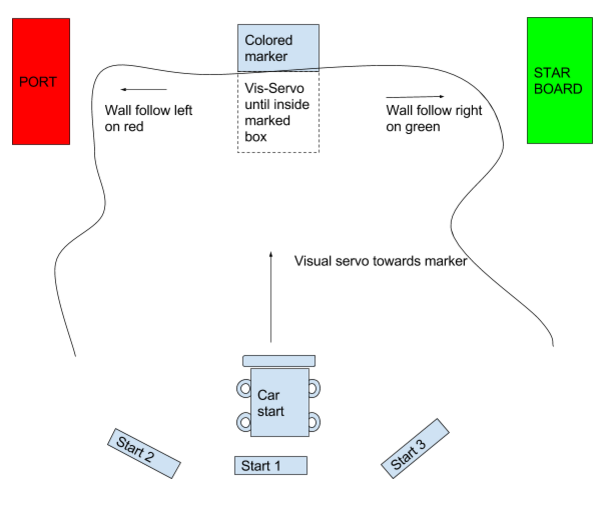
\includegraphics[scale=.42]{visual_servo.png}
\caption{Challenge diagram \cite{vs-handout}} 
\end{figure}
\subsection{Approach}
We started with getting a good blob detections algorithm, then worked on a simple but effective visual servoing method that could then transition into the wall following modified from last week. We split up the task into a blob detection node, a blob follow node, and a turn node in order to facilitate testing and so we could split up the work effectively. 
\subsection{Process}
\par We first focused on the image detection, then split people up to work on various aspects of the visual servoing and wall following. In a lab session, we worked individually on each getting good blob detection. Everyone in the team put the working parts of their code together and we built off the final one. We split up the team, giving different people different tasks. Some members of the group worked on a visual servoing method using a bang bang method based on height and x position of the blob. If the blob was too far it would go forwards, if it was close enough it would stop. If the x position of the blob was on the right side of the screen, the robot turned right. If the x position of the blob was on the left side, the robot turned left. As expected with a bang bang controller, it was jerky and when we were close to the target, it had trouble getting oriented because if it was a little off center, it would turn back too much and be stuck in an oscillation cycle. We decided to implement a PID controller into our visual servo, which helped with this issue. 
\par While some people were working on that, others worked on taking our wall-follow code from last week and modifying it and optimizing it for our situation. We didn’t focus on tuning this part too much because we knew it functioned from last week. Another sub-group worked on setting up the structure of the task and how the nodes would communicate. We were able to successfully integrate them together. Due to miscommunication, we realized that no one had programmed the turn for when it got to the wall. We struggled to get that part working for the race because of lack of testing time. 
\subsection{Results}
At the very last minute we were able to get the robot to turn and follow properly when it got to the wall. Unfortunately, it only worked on the green side because we figured out later that there was a bug in our code where the isGreen variable we were modifying was a local variable. Then during the race, our robot didn’t move probably due to lack of battery. After we charged it, the program did not work the same way and the gears had a glitch, so unfortunately we couldn’t finish. Importance of testing
\section{Week 3}
\subsection{Technical goals}
Our goal was to use reactive-based planning-based on what the robot can see locally in order to explore unbounded space while avoiding obstacles. We also had to detect blobs along the way and save the picture with the blob color and locations indicated. To add on from the image detection from last week, additional colors to detect were added(blue and yellow), and there was a challenge task to detect images of Ari, Sertac, a cat, and a robot. 
\subsection{Approach}
Based on the open-ended nature of this week’s assignment, we had a team meeting where we discussed a lot of possible methods for obstacle avoidance and ways to take the shortcut. We first focused on ways to get around without obstacles. We had different people explore different ideas. In the end, we ended up using a potential field method that we learned about in a lecture, which was the most effective.
\subsection{Process}
Here are the methods we explored in the order we considered them
\subsubsection{Right wall follow}
If there are no obstacles and we’re not supposed to take the shortcut, we thought that a simple wall follow should be sufficient. However, we found that because of the sharp corner, it wouldn’t be an option. As the robot approached the corner, it could never determine that it should turn until it had already run into the wall, since the robot looks out to the side and not directly in front of it. After we adjusted the field of vision to angled further up front, it was able to turn at the corner only at very low speeds. 
\subsubsection{Equal Distance wall following}
Assuming there are no obstacles, an effective way to take the shortcut would be to simply follow the wall on both sides by trying to keep the distances on the left and the right the same. When the robot got to the shortcut, it would see a large spike in the laser reading for the left side and therefore turn left to account for it. However, it was determined that this model would break down with obstacles. 
\subsubsection{Obstacle detect}
Look ahead and if obstacles are detected on the left side, take the right lane and vice versa. If both left lane and right lane have obstacles, take the center lane. The idea of changing the desired distance of the wall follow based on where the obstacles were was solid, but too many assumptions were made in the model
\subsubsection{Left/Right Wall Follow}
If there are no obstacles, follow the left wall the whole time, then switch to following the right wall when there is the shortcut to ensure that the robot takes the long way across.
\subsubsection{State machine}
We explored enough options for the case of wanting to take the shortcut and not taking the shortcut, along with how to avoid obstacles that based on where it is, that we could incorporate them all into a state machine. [Possible elaborate]
\subsubsection{Open space}
Use the scanner to find the largest contiguous open space and go there. This method could work well, especially for avoiding obstacles. We ran out of testing time to try it out, however. 
\subsubsection{Potential field}
The potential field method uses the idea of charges attracting and repelling to control the robot. The robot is repelled from obstacles, but also repelled from behind so it continues to move. We ended up this method because it was the most robust.

For the blob detections, we used the version we made last week and added in the new colors. We came up with two possible solutions that we could have had working with more time. The first one was to average the HSV values of the pixels in each of the challenge images and hope that they are different enough that we could distinguish them. This would be messed up in different lightings, but since we aren’t penalized for incorrect labelling, we thought it could be worth it. The second method would to do some sort of statistical analysis of the HSV values of the pixels of the original images. Then, we could find the distribution for the images from the ZED camera and compare them to find the closest match. 
\subsection{Results}
In the final challenge, we used the potential field method. We ran out of time to execute the challenge images and we weren’t able to tune the color values well, so we missed a lot of colors in the actual challenge. We should have spent more time tuning the colors instead of focusing on the challenge images. We ended up coming in 3rd place with 36 points, which came from detecting four blobs and having two collisions. 

\section{Week 4}
\subsection{Technical goals}
This week was dedicated to preparation for the Grand Prix Challenge race, but in addition there were two tech challenges that would be informally showcased. 
\subsubsection{Tech Challenge 1}
In the first tech challenge, the robot had to publish blob detections while it explored an unstructured space with obstacles.  
\subsubsection{Tech Challenge 2}
In the second tech challenge, the robot had to go along the racetrack and look for a colored blob that would be located at a forked intersection. A green blob would indicate an open shortcut that the robot could take while a red blob would indicate that the shortcut was blocked and the robot has to take a longer way around. 
\subsubsection{Grand Prix Race}
[Get a picture]
\subsection{Approach}
how did we set about work and why
\subsection{Process}
Step by step process of what we did
\subsection{Results}
Results - what was tested, what was accomplished
\subsubsection{Time trial}
Our team ranked 1st out of all 9 teams in the time trial with the following times:
    \begin{table}[!hbt]
        % Center the table
        \begin{center}
        % Title of the table
        \caption{Time Trial Results}
        % Table itself: here we have two columns which are centered and have lines to the left, right and in the middle: |c|c|
        \begin{tabular}{|c|c|c|}
            % To create a horizontal line, type \hline
            \hline
            % To end a column type &
            % For a linebreak type \\
			\textbf{Lap \#} & \textbf{Color of blob} & \textbf{Time} \\
			\hline
            1 & Green & 28.93\\
            \hline
            2 & Red & 33.46 \\
            \hline
            3 & Red & 33.28\\
            \hline
        \end{tabular}
        \end{center}
    \end{table}
    \begin{table}[!hbt]
        % Center the table
        \begin{center}
        % Title of the table
		\caption{Final Grand Prix Results}
        % Table itself: here we have two columns which are centered and have lines to the left, right and in the middle: |c|c|
        \begin{tabular}{|c|c|}
            % To create a horizontal line, type \hline
            \hline
            % To end a column type &
            % For a linebreak type \\
			\textbf{Color} & \textbf{Time} \\
			\hline
            Green & 28.00 \\
            \hline
            Red & 38.20 \\
            \hline
        \end{tabular}
        \end{center}
    \end{table}
\section{Conclusion}
Summarize goals, results, failures \\
What did we learn \\ 
What we’ll do differently next time \\

\section{How to do stuff}
    The report can be written in \LaTeX{} or Microsoft Word, but \LaTeX{} is definitely preferred.
    Its appearance should be as close to this document as possible to achieve consistency in the proceedings.

    % You can cite a book or paper by using \cite{reference}.
    % The references will be defined at the end of this .tex file in the bibliography
    References should be cited as numbers, and should be ordered by their appearance (example: ``... as shown in \cite{HOP96}, ...'').
    Only references that are actually cited can be listed in the references section.
    The references' format should be evident from the examples in this text.

    References should be of academic character and should be published and accessible.
    Your advisor can answer your questions regarding literature research.
    You must cite all used sources.
    Examples of good references include text books and scientific journals or conference proceedings.
    If possible, citing internet pages should be avoided. In particular, Wikipedia is \emph{not} an appropriate reference in academic reports.
    Avoiding references in languages other than English is recommended.

    % You can reference tables and figure by using the \ref{label} command. Each table and figure needs to have a UNIQUE label.
    Figures and tables should be labeled and numbered, such as in Table~\ref{tab:simParameters} and Fig.~\ref{fig:tf_plot}.

    % This is how you define a table: the [!hbt] means that LaTeX is forced (by the !) to place the table exactly here (by h), or if that doesnt work because of a pagebreak or so, it tries to place the table to the bottom of the page (by b) or the top (by t).
    \begin{table}[!hbt]
        % Center the table
        \begin{center}
        % Title of the table
        \caption{Simulation Parameters}
        \label{tab:simParameters}
        % Table itself: here we have two columns which are centered and have lines to the left, right and in the middle: |c|c|
        \begin{tabular}{|c|c|}
            % To create a horizontal line, type \hline
            \hline
            % To end a column type &
            % For a linebreak type \\
            Information message length & $k=16000$ bit \\
            \hline
            Radio segment size & $b=160$ bit \\
            \hline
            Rate of component codes & $R_{cc}=1/3$\\
            \hline
            Polynomial of component encoders & $[1 , 33/37 , 25/37]_8$\\
            \hline
        \end{tabular}
        \end{center}
    \end{table}

    % If you have questions about how to write mathematical formulas in LaTeX, please read a LaTeX book or the 'Not So Short Introduction to LaTeX': tobi.oetiker.ch/lshort/lshort.pdf

    % This is how you include a eps figure in your document. LaTeX only accepts EPS or TIFF files.
    \begin{figure}[!hbt]
        % Center the figure.
        \begin{center}
        % Include the eps file, scale it such that it's width equals the column width. You can also put width=8cm for example...
        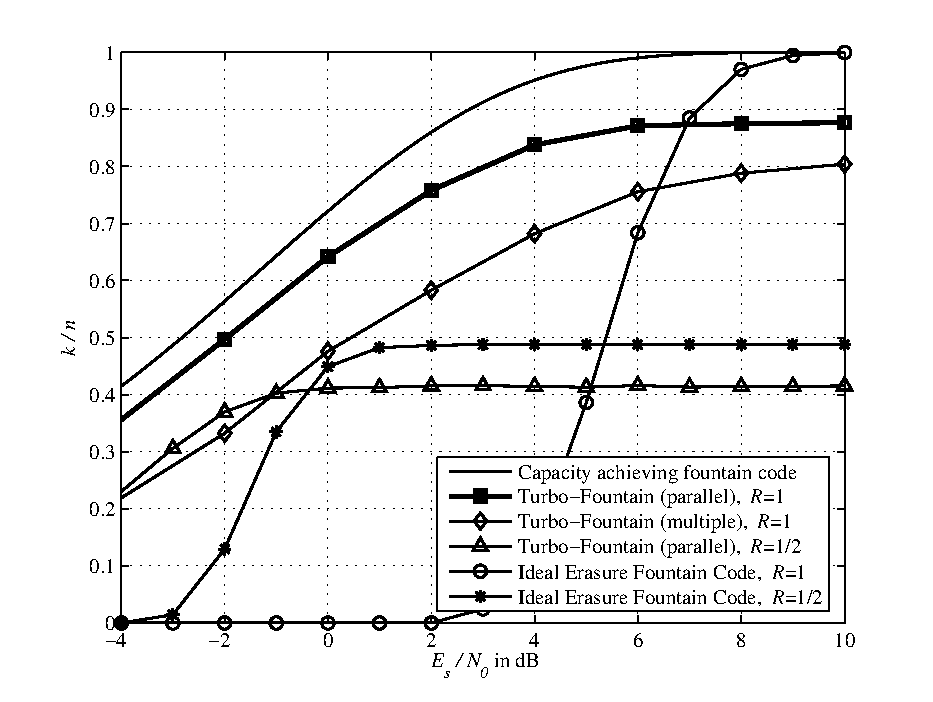
\includegraphics[width=\columnwidth]{plot_tf}
        % Create a subtitle for the figure.
        \caption{Simulation results on the AWGN channel. Average throughput $k/n$ vs $E_s/N_0$.}
        % Define the label of the figure. It's good to use 'fig:title', so you know that the label belongs to a figure.
        \label{fig:tf_plot}
        \end{center}
    \end{figure}

\section{Filling this page}
    Gallia est omnis divisa in partes tres, quarum unam incolunt Belgae, aliam Aquitani, tertiam qui ipsorum lingua Celtae, nostra Galli appellantur. Gallos ab Aquitanis Garumna flumen, a Belgis Matrona et Sequana dividit. Horum omnium fortissimi sunt Belgae, propterea quod a cultu atque humanitate provinciae longissime absunt, minimeque ad eos mercatores saepe commeant atque ea quae ad effeminandos animos pertinent important, proximique sunt Germanis, qui trans Rhenum incolunt, quibuscum continenter bellum gerunt. Qua de causa Helvetii quoque reliquos Gallos virtute praecedunt, quod fere cotidianis proeliis cum Germanis contendunt, cum aut suis finibus eos prohibent aut ipsi in eorum finibus bellum gerunt. Eorum una, pars, quam Gallos obtinere dictum est, initium capit a flumine Rhodano, continetur Garumna flumine, Oceano, finibus Belgarum, attingit etiam ab Sequanis et Helvetiis flumen Rhenum, vergit ad septentriones. Belgae ab extremis Galliae finibus oriuntur, pertinent ad inferiorem partem fluminis Rheni, spectant in septentrionem et orientem solem.

\section{Conclusion}
    This section summarizes the paper.
\nocite{5}
% Now we need a bibliography:
\bibliographystyle{unsrt}
\bibliography{report}

% Your document ends here!
\end{document}
